\documentclass{article}
\usepackage[spanish]{babel} %Definir idioma español
\usepackage[utf8]{inputenc} %Codificacion utf-8
\usepackage{amssymb, amsmath, amsbsy, wasysym}
\usepackage{multirow} % para tablas
\usepackage{graphicx}
\usepackage[dvipsnames]{xcolor}
\title{Práctica 4}
\author{Emmanuel Peto Gutiérrez}
\begin{document}
\maketitle

\section{Introducción}

Esta práctica consiste en implementar los siguientes algoritmos de ordenamiento:
\begin{itemize}

\item[1.] Selection Sort
\item[2.] Insertion Sort
\item[3.] Merge Sort
\item[4.] Quick Sort

\end{itemize}

\section{Descripción}

\subsection{Entrada}

El programa a implementar recibe como entrada en los argumentos de la linea
de comandos (ejecutando desde la carpeta ``src''):

\begin{itemize}
\item[1.] \textbf{Nombre} de la imágen a procesar (debe encontrarse en la carpeta resource).

\item[2.] {\bf Velocidad}, se trata de un número entero que indica el numero de iteraciones que ocurriran antes de actualizar la interfaz grafica (Entre más grande sea el numero, menos actualizaciones de la interfaz. Y por lo tanto, mayor velocidad).

\item[3.] {\bf Algoritmo} a utilizar para el ordenamiento. Las unicas opciones son: ``selection'', ``insertion'', ``merge'' y ``quick''.

\end{itemize}

Por ejemplo, para ordenar la {\bf imagen1} a una velocidad de {\bf 40}, utilizando {\bf insertion} sort:

\begin{center}
java sort.Main imagen1 40 insertion
\end{center}

\subsection{Salida}

Una vez que se ha leido la imágen de entrada.

\begin{center}

\includegraphics[scale=0.25]{ink}
\end{center}

Los pixeles de dicha imágen deben ser intercambiados de manera aleatoria
para generar una imágen con los mismos pixeles, pero en distinto orden.

\begin{center}

\includegraphics[scale=0.25]{ink2}
\end{center}

Ya obtenida la imagen ``revuelta'', debe entonces aplicarse el algoritmo de ordenamiento indicado en la linea de comandos para reconstruir la imagen y regresarla a su estado original.

Las iteraciones de los algoritmos de ordenamiento deben ser visibles en la interfaz grafica en tiempo real. Esto con el fin de poder observar el comportamiento de los algoritmos de manera visual.

\begin{center}
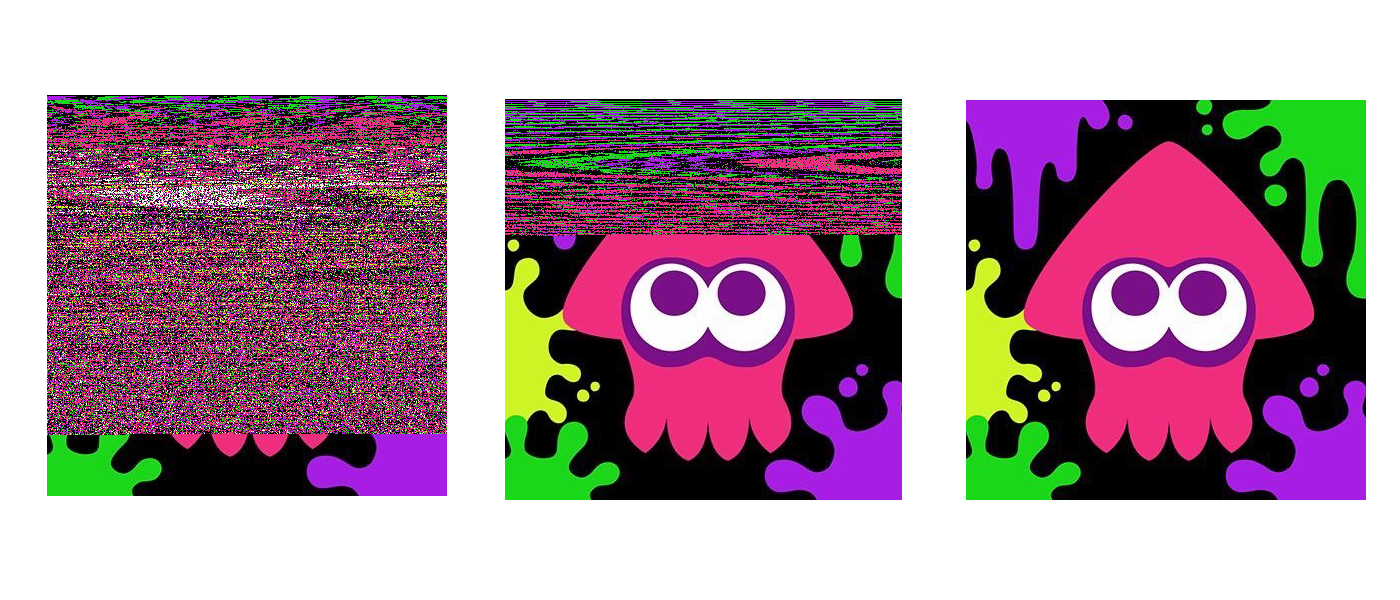
\includegraphics[scale=0.25]{ink3}
\end{center}

Se proporciona un código base para manipular las imágenes, de manera que sólo queda pendiente implementar los algoritmos de ordenamiento en la clase \textbf{Sort.java}. Tienen que completar las funciones \emph{selectionSort()}, \emph{insertionSort()}, \emph{mergeSort()} y \emph{quickSort()}.

En dicha clase se proporciona un ejemplo con la implementación de Bubble Sort y el uso del método \emph{update} en conjunto con la variable \emph{framerate} para el manejo de las actualizaciones de la interfaz gráfica.

\section{Entrega}

\begin{itemize}
\item Deben entregarlo como un archivo comprimido de una carpeta con el mismo nombre.
\item La carpeta debe ser: \textbf{Practica4\_ApellidopaternoApellidomaterno}. Por ejemplo \textbf{Practica4\_PetoGutierrez}.
\item Su carpeta debe contener un archivo \emph{readme} que contenga: número de cuenta, nombre completo, 
correo y las instrucciones para compilar y ejecutar su programa(se recomienda un \emph{Makefile}).
\item Si su carpeta contiene un ejecutable(como *.jar) enviarlo como un enlace de dropbox o drive.
\item El asunto debe ser: \textbf{[AAlgoritmos]Practica4}.
\item El correo al que enviarán la práctica es: \emph{empg014@ciencias.unam.mx}
\end{itemize}

La fecha de entrega es el jueves \textbf{17 de octubre}.

\end{document}

